\chapter{はじめに}
\thispagestyle{fancy}
\setcounter{page}{1}
\renewcommand{\thepage}{\arabic{page}}

\section{研究背景}
近年、エンターテインメントコンピューティングが注目され,日本の主要産業の一つとなった.

従来の工学は物質的な豊さを求められてきたが,それが飽和しつつある昨今,
精神的な豊さを求めるため新しいエンターテインメントを創造するための
技術とコンテンツの研究を行う研究分野がエンターテインメントコンピューティングである.
その中でも本研究では,プロジェクションマッピングに着目した.

プロジェクションマッピングは,プロジェクターを使用して空間と映像を合成することにより、
新しい空間を作成する技術である。
多くの人がダンサーのパフォーマンスとプロジェクションマッピングを組み合わせた素晴らしい
世界を作り出す作品に魅了されたことがあるだろう.
ただし、これらの作業では、パフォーマーがプロジェクションマッピングの画像オブジェクトの座標に
正確に動きを合わせる必要があるが、これは多くの人に取って困難であると考える.

本研究では、プロジェクションマッピングを見る人々だけでなく,パフォーマーも楽しませるために,
パフォーマーの動きに応じてインタラクティブに変化する参加型のプロジェクションマッピングを提案する.



\section{プロジェクションマッピングの歴史}
プロジェクションマッピングは最新の技術と思う人も多いだろうがそうでは無い.
ベースにある考え方や手法は実は古くから様々な場所で行われていた.
プロジェクターが様々なクリエイターの手に渡った時から,それを使った新たな表現を求め,
その流れの中で15年以上前から自然発生的に生まれてきた.特に舞台やイベント,
ビデオアートやインスタレーションといわれる表現の世界では早くから取り組まれ,
メディアアートとしても試行錯誤が行われている.

注目を集めるようになった理由として,まず機材や映像技術の発達である.
特に高輝度のプロジェクターがクリエイターの手に届くようになり,
ヨーロッパで建築物への大規模なプロジェクションが試みられ始めると,
それらの作品のスケールや完成度から大きなインパクトを与えた.

次に,インターネットが普及してきた背景が挙げられる.YouTubeなどで急速に話題を集め始めた.
近年の日本でも,各種メディアで数多く紹介され,イベントやアミューズメントパーク,
季節のイベント等でも使用され,親しまれるようになってきている\cite{hoge}.



\section{プロジェクションマッピングの実用例}
まず,建物への投影だ.図\ref{disney}に,東京ディズニーランドで2014年5月から2017年11月まで行われた「Once upon a time」を示す.
シンデレラ城にマッピングをし,驚きと感動を届けた.
現在もシンデレラ城で新たなプロジェクションマッピングが行われている\cite{hoge}.
また,図\ref{rio}の2016年8月に開幕した「リオオリンピック」開閉会式でもプロジェクションマッピングは行われた. 
2万ルーメンのプロジェクターをメインに333台のプロジェクターが使用された.
開会式では、プロジェクションマッピングを駆使した美しい映像演出が反響を呼び、
南米初開催となったオリンピックを強く印象づけた\cite{hoge}.

次にライブやコンサートなどのイベントである.安室奈美恵は,二段構えの垂直のセット,
6面の縦長のビジョンを用い,ダンサー3人とプロジェクションマッピングが重なるような演出を行った\cite{hoge}.
また,Perfumeがフランス・カンヌで6月に開催された世界最大の広告祭
「カンヌライオンズ 国際クリエイティビティ・フェスティバル」でのパフォーマンスで,
プロジェクションマッピングを行った.3人がまとう真っ白な衣装がスクリーンとなり,
次々と色鮮やかなグラフィックが映し出された\cite{hoge}.
このようにステージの背景だけでなく,アーティスト自身に投影を行うような例もある.

また,プロジェクションマッピングは,エンターテインメント分野だけでなく,
手術をリアルタイムでナビゲーションする装置[7]など,医療分野でも応用されている.


\clearpage

\begin{figure}[t]
  \centering
  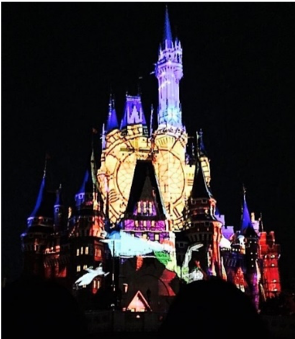
\includegraphics[width=8cm]{image/disney.png}
  \caption{東京ディズニーランド Once upon a time}
\label{disney}
\end{figure}

\begin{figure}[b]
    \centering
    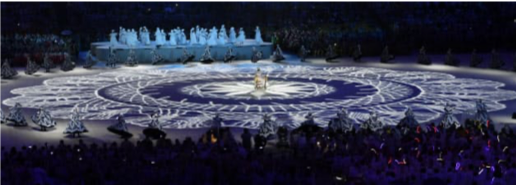
\includegraphics[width=8cm]{image/rio.png}
    \caption{リオオリンピック}
  \label{rio}
\end{figure}

\clearpage

\begin{figure}[t]
    \centering
    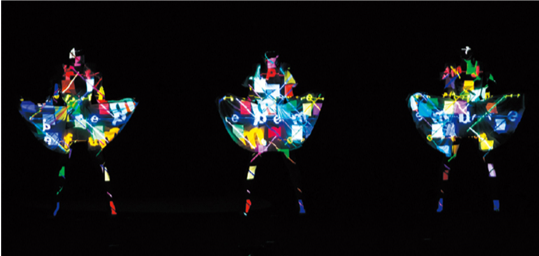
\includegraphics[width=10cm]{image/perfume.png}
    \caption{Perfume カンヌライオンズ 
    \protect\linebreak 国際クリエイティビティ・フェスティバル\cite{hoge}}
  \label{perfume}
\end{figure}

  



\clearpage
\section{本論文の構成}
本論文の以下の構成は次のようになっている.
第2章では,関連研究を紹介する.
第3章では,Twitterアカウントの評価を行う手法の提案を行う.
第4章では、Twitterの主な機能とAPIについて説明する.
第5章では,評価実験について示す.
第6章では,評価結果について示す.
第7章では,本研究の提案手法の考察を述べる.
第8章では,まとめと今後の課題について述べる.
なお、付録として本研究で用いたソースコードを加えた。
